\section{Introduction}
In this chapter NoSQL databases are firstly introduced, described in their main characteristics and a general classification is provided. In section \ref{sec:common-language} are listed some of the solutions that have been developed trying to define a common interface to interact with different NoSQL databases.

\noindent In section \ref{sec:jpa} is also described the JPA interface and JPQL, the querying language used for issuing queries. In section \ref{sec:cpim} the CPIM library is introduced as a tentative of defining a common interface to interact with different vendors in PaaS environments (which includes accessing their NoSQL solution).

\section{NoSQL databases}
\label{sec:nosql}
NoSQL databases have recently became popular, due to the inadequacy of traditional RBDMSs to guarantee adequate performances with respect to the new application requirements that in these years have outlined. These requirements primarily concern the ability of handling huge amount of unstructured or semi-structured data.

\noindent RDBMSs provide a general-purpose solutions that balance the various requirements of applications, but they works well for application handling structured data and for applications that have strict requirement on consistency (as they guarantee full ACID consistency). Examples are business or administrative application since RBDMSs were born more than 30 years ago, when these were the most common applications.

\noindent NoSQL databases have emerged as a way to store unstructured, semi-structured data and other complex objects such as documents, data streams, and graphs. Moreover they provide the capabilities for handling huge amount of those kind of data, while providing reasonable performance.
This is done primarily by recognizing that many modern applications such as social networks, does not need full ACID compliance. Indeed, full ACID compliance may not be important to a search engine that may return different results to two users simultaneously, or to Amazon when returning sets of different reviews to two users.

\subsection{NoSQL characteristics}
Due to the different approaches that NoSQL database put in place to meet the new application requirements, there is no a unique NoSQL definition but since all of them provides similar features, we can say that NoSQL databases are distributed databases with flexible data models aimed to provide: horizontal scalability, fault tolerance and high availability.

\noindent As distributed systems, NoSQL databases are governed by the CAP theorem; it states that, in a distributed system, we can only have two out of three of the following guarantees:
\begin{itemize}
\item \textbf{Consistency}, a read is guaranteed to return the most recent write for a given client;
\item \textbf{Availability}, a non-failing node will return a reasonable response within a reasonable amount of time (no error or timeout);
\item \textbf{Partition tolerance}, the system will continue to function when network partitions occur.
\end{itemize}

\noindent As a result, we can have a distributed system with only one of these three combination of properties: CA, CP or AP.

\noindent Given that networks aren't completely reliable, partitions must be tolerated; according to the CAP theorem, this means that essentially two are the remaining valid options: Consistency and Availability.

\noindent For those reasons, while RDBMS scale very well vertically, and thus adding computational power to the node, they do not scale particularly well horizontally and thus through sharding. This is because RDBMS guarantee ACID properties, and thus consistency, while for sharding, the system should be tolerant to partition but, being a distributed system, this means, in terms of the CAP theorem, that RDMBS cannot guarantee availability. In contrast, NoSQL database sacrifice consistency for the sake of efficiency an thus, with respect to the CAP theorem, they can guarantee both partition tolerance and availability, properties that permit them to scale well horizontally by means of sharding.

\noindent The decision of neglecting consistency, makes NoSQL databases no more ACID compliant, to highlight this fact, they are said to be BASE compliant, where BASE is the acronym of:
\begin{itemize}
\item \textbf{Basically Available}, which indicates that the system does guarantee availability, in terms of the CAP theorem;
\item \textbf{Soft state}, which indicates that the state of the system may change over time, even without input;
\item \textbf{Eventual consistency}, which indicates that the system will become consistent over time, given that the system doesn't receive input during that time.
\end{itemize}
\noindent Those properties are perfect for certain type of web application, as pointed out previously, and permits to NoSQL databases to guarantee valuable performance in the scenario of Web 2.0 applications requirements.

\subsection{NoSQL classification}
Many NoSQL datastore has been developed and each of them manage data in different ways depending on the requirements it tries to address and how it ranks as compared to the CAP theorem.
There is not a general classification for NoSQL databases, many are the method that can be used to classify them: the data model, the architecture, the sharding or replication methods. We will consider the classification based on the data model since is the most common method used to categorize them.

\noindent Accordingly to the meta model, NoSQL databases can be classified in four groups: key-value, column-oriented, document-oriented and grap-based.

\paragraph{Key/Value stores} This kind of databases are very similar to data structures such as Maps or Hashtables, indeed, data are stored as values which are then associated to a key. This databases are thus completely schema-free and can easily store non structured data.This permits to write huge amounts of data and even to horizontally distribute them (sharded) among the nodes of the system.
Examples of this kind of databases are Redis\footnote{\url{http://redis.io}} and Voldemort\footnote{\url{http://www.project-voldemort.com}}.

\paragraph{Column-oriented databases} Those databases are mainly inspired by the Google Big Table \cite{paper:bigtable} data model, and are designed for storing data tables as sections of columns of data, rather than as rows of data. Hence, entity properties are stored in \textit{Columns} that are then grouped in \textit{Column families}; rows are identified by a key and composed by a set of column, each row can have a different set of columns with respect to other rows to be able to persist even semi-structured and unstructured data.
This kind of databases allows great scalability options as they can both scale horizontally (sharding), by distributing rows, and vertically, by distributing column families among the node of the system.

\noindent Examples of this kind of databases are Cassandra\footnote{\url{http://cassandra.apache.org}} and HBase\footnote{\url{http://hbase.apache.org}}.

\paragraph{Document-oriented databases} Document-oriented databases are designed for storing, retrieving, and managing document-oriented data. These systems are designed around an abstract notion of a Document identified in the database via a unique key. 
Document database typically offer a query language that allows the user to retrieve documents based on their content because they extract and index all kinds of meta-data and usually also the entire content of the documents. 
Documents can be stored in many different ways such as JSON, BSON, YAML or XML.

\noindent An example of this kind of database is MongoDB\footnote{\url{http://www.mongodb.org}} and Couchbase\footnote{\url{http://www.couchbase.com}}.

\paragraph{Graph databases}  Graph databases are databases that uses graph theory to represent the data.
Persisted entities are represented by nodes; each node maintains the information about the entity it represents by storing them into properties, while edges can be used to represent relationships among the entities.

\noindent An example of this kind of database is Neo4j\footnote{\url{http://neo4j.com}}.

\newparagraph As we write there are more than 150 \cite{online:nosql-database.org} different NoSQL databases and not all of them can be strictly categorized in one of the previous classification. Furthermore other solutions trying to propose multiple data models are being developed. Example of those systems are: OrientDB\footnote{\url{http://www.orientechnologies.com}}, an hybrid solution which data model span across graph and document databases and ArangoDB\footnote{\url{https://www.arangodb.com/}}, which data model is an hybrid of document, graph and key-value data models.

\section{Approaches for offering a common language over NoSQL}
\label{sec:common-language}
The variety of NoSQL systems is huge and the lack of a a common standardized language for NoSQL databases is a great concern for companies interested in adopting any of these systems, applications and data are expensive to convert and competencies and expertise acquired on a specific system get wasted in case of migration. 
Also, most of the NoSQL interfaces support a lower level of interaction than SQL, which appear to be a step back with respect to DBMS.

\subsection{SQLifying NoSQL}
A fist approach that is emerging is the \textit{SQLfication} of NoSQL databases.
NoSQL vendors, in order to overcome the problem of industry wasting the expertise maturated over SQL systems, started to create, around their NoSQL solutions, SQL-like wrappers,  which typically offer different features with respect to those of a traditional relational database query language, but maintaining a grammar similar to that of SQL.

\noindent For example Google App Engine Datastore, provides GQL, a SQL-like language for retrieving entities or keys from Datastore.
Other NoSQL database, such as Cassandra (with CQL), or OrientDB, provide  such type of SQL-like language support natively.

\newparagraph There exist also some independent projects that aim to create such kind of SQL-like languages upon existing NoSQL databases.

\subsubsection{Apache Phoenix} 
Apache Phoenix \cite{online:apache-phoenix} aims to become the standard means of accessing HBase data through a well-defined, industry standard API.
It is a relational database layer over HBase delivered as a client-embedded JDBC driver over HBase data. Apache Phoenix takes standard SQL queries, compiles them into a series of HBase scans, and orchestrates the running of those scans to produce regular JDBC result sets. 

\subsubsection{UnQL}  
Unstructured Data Query Language \cite{online:unql}, or UnQL (pronounced “Uncle”), is a tentative to bring a familiar and standardized data definition and manipulation language to the NoSQL domain. The project was started in 2011 by the joint effort of Couchbase and SQLite.

\noindent After the project was started, and after some burst of activity, the project came to a hold. So it seems, that at least as a project UnQL has been a failure. 

\subsection{Meta-model approaches}
Another way that has been investigated in order to achieve interoparability,  is trying to abstract from the data model by spotting common concepts in the data model of various NoSQL solutions, in order to define a more general meta-model that can offer an common interface to store data.

\subsubsection{Apache MetaModel}
The aim of Apache MetaModel is to provide a common interface for discovery, exploration of metadata and querying of different types of data sources \cite{online:apache-metamodel}.

\noindent The peculiarity of this project is that it does not only provide support for NoSQL database (such as CouchDB, MongoDB, Hbase, Cassandra and ElasticSearch) but also for relational databases (such as PostgreSQL, MySQL, Oracle DB and SQL Server) and even for various raw data format (such as JSON, XML and CSV files).
 
\noindent The defined meta-model gives the ability to add data sources at run-time and provides a type-safe SQL-like API. An example for a table creation is reported in the code \ref{code:apache-metamodel-table}, the meta-model defines a different semantic for the concept of \textit{table} depending on the underlying storage technology. For example, for JDBC it issues a CREATE TABLE statement to the database, for a CSV file, it creates or overwrites the file and for MongoDB, it creates a new collection in the MongoDB database.

\begin{lstlisting}[language=Java, caption=Apache MetaModel example, label=code:apache-metamodel-table]
// CREATE a table
Table table = callback.createTable("Employee")
    .withColumn("id").ofType(INTEGER)
    .withColumn("name").ofType(VARCHAR).execute();
\end{lstlisting}
            
\subsubsection{SOS Platform}
The SOS (Save Our Systems) Platform \cite{paper:sos-platform} is an academic project developed by Unversit\`{a} Roma Tre.

\noindent The platform achieves interoperability among NoSQL databases by defining a common interface through a meta-layer of abstraction used to maintain entities information. Database specific handlers read the meta-layer and translate the meta-operations to database-specific operations that are finally performed over the database instance.
The architecture is shown in figure \ref{fig:sos-architecture}.

\begin{figure}[tbh]
  \centering
  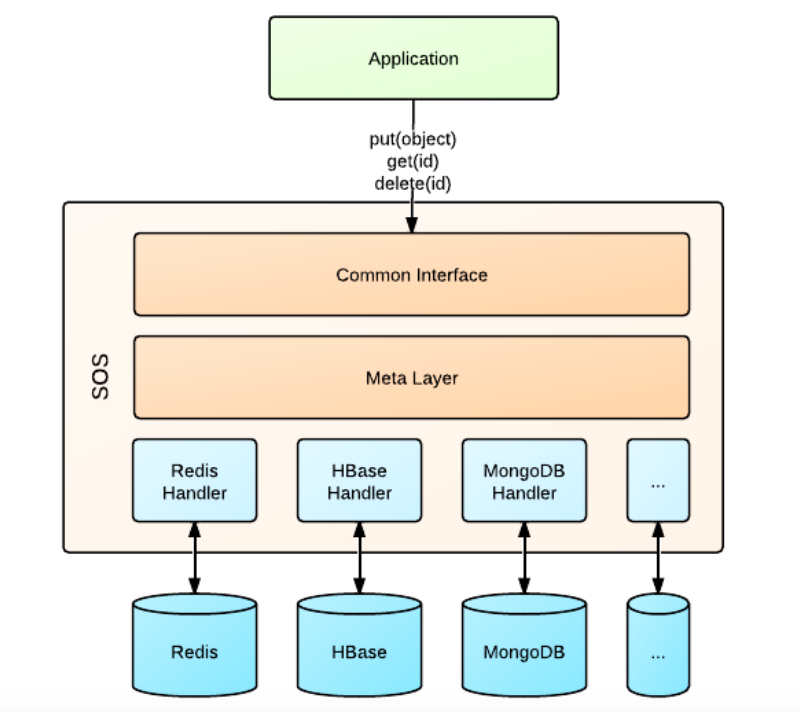
\includegraphics[width=9cm]{images/sos_architecture}
  \caption{SOS architecture \cite{paper:sos-platform}}
  \label{fig:sos-architecture}
\end{figure}

\noindent The supported NoSQL databases are: Hbase to represent Column-based databases, MongoDB to represent Document-oriented databases and Redis for Key/Value stores. 
\noindent The meta-layer exploit the data model similarities and is actually very simple; it is composed by three main constructs: Struct, Set and Attribute.
Attributes contain simple values, such as Strings or Integers; Structs and Sets are instead complex elements whose values may contains both Attributes and Sets or Structs as well.
Each database is represented as a Set of collections whose is a Set itself, containing an arbitrary number of objects. Each object is identified by a key that is unique in the collections it belongs to.

\subsection{ORM approaches}
Object Relational Mapping (ORM) solutions came into existence to solve the  \textit{object-relational impedance mismatch} problem, that is often encountered when a relational database management system (RDBMS) is being used by a program written in an object-oriented programming language or style; ORM were thus primarily introduced to ease the interaction with RDBMS.

\noindent Each ORM solution had its own API and object query language (like HQL for Hibernate) which made it difficult for programmers to switch from one framework to another. As a result, efforts were made to make standards and specifications for this tools. 

\noindent Today ORM have become the standard way that developers use to interacts with RDBMS due to the great advantages they bring, such as the ability to change RDBMS without modifications in the application code.
The advantages that ORM led to RDBMS made people think that this approach, or a similar one, should be applied to NoSQLs too. 
Furthermore people lack in-depth knowledge of NoSQL and even if they do, their knowledge is limited to a couple of them. For this reasons the ORM approach seems to fit perfectly since they gives to developers a way to interact with NoSQL in a way they are comfortable with, leaving the complexity of NoSQLs to the ORM.

\subsubsection{The JPA interface}
\label{sec:jpa}
Since many of the ORM solutions have their roots in the JPA interface, an ORM standard for Java based applications, is worth describe it.

\newparagraph The Java Persistence API \cite{book:projpa2} was first released as part of Enterprise JavaBeans 3.0 in 2006. As a more general-purpose object-relational mapping facility, it was quickly recognized as such, and was expanded at the request of the community to support use in Java SE environments as well as in the other Java EE container types.

\noindent The Java Persistence API provides an object/relational mapping facility to Java developers for managing mainly relational data within Java applications. Java Persistence consists of three areas:
\begin{itemize}
\item the Java Persistence API;
\item object/relational mapping meta-data;
\item the query language.
\end{itemize}

\noindent Mapping meta-data are defined by the user as Java annotations upon the classes that he wants to map to the underlying database.
The user annotates classes representing entities; typically, an entity represents a table in a relational database, and each entity instance corresponds to a row in that table. Entities are managed by the entity manager; the \texttt{EntityManager} API creates and removes persistent entity instances, finds entities by their primary key, and allows queries to be run on entities. 
The \texttt{EntityManager.createQuery} and \texttt{EntityManager.createNamedQuery} methods are used to query the database using Java Persistence query language queries; the only difference among them is that the latter permits to define queries statically, within the entity meta-data, through a specific annotation and referencing it later by name.

\noindent A \textit{peristence unit} is set to all entity classes managed by the \texttt{EntityManager} instance.
Persistence units are defined by the \textit{persistence.xml} configuration file. Each persistence unit is identified by a name, that is unique across the persistence units scope. 

\newparagraph The JPA supports two methods for expressing queries, in order to retrieve entities and other persistent data from the database: query languages and the criteria API. The primary query language is Java Persistence Query Language (JPQL), a database-independent query language that operates on the logical entity model, as opposed to the physical data model. Queries may also be expressed in SQL to take advantage of the underlying database. The criteria API provides an alternative method for constructing queries based on Java objects instead of query strings.
An example of defining the same query with the two approaches is shown in the code \ref{code:jpa-queries}.
the JPA approach.

\begin{lstlisting}[language=Java, caption=Create queries with JPA, label=code:jpa-queries]
// using criteria API
CriteriaBuilder cb = em.getCriteriaBuilder();
CriteriaQuery<Employee> query = cb.createQuery(Employee.class);
Root<Employee> e = query.from(Employee.class);
query.select(e);
  
// using JPQL
TypedQuery<Employee> query = em.createQuery("SELECT e FROM Employee e");
\end{lstlisting}

\noindent JPQL has its roots in the Enterprise JavaBeans Query Language (EJB QL) that was first introduced in the EJB 2.0 specification to allow developers to write portable ``find'' and ``select'' methods, for container-managed entity beans. It was based on a small subset of SQL and it introduced a way to navigate across entity relationships both to select data and to filter the results.
JPQL was then introduced as part of the JPA to significantly extend EJB QL, thus eliminating many of its weaknesses, while preserving backward compatibility.

\subsubsection{Kundera}
Kundera \cite{online:kundera} is an open source project started by \textbf{Impetus Inc.} an India based tech company active in Big Data and Cloud engineering.
Kundera provides a JPA 2.1 compliant object-datastore mapping library for NoSQL datastores leveraging the existing NoSQL database libraries, and builds on top of them a wrapper compliant to the JPA specifications.

\noindent The main advantage of the Kundera approach is that, using a well known and defined interface, developers do not need to learn a new framework, furthermore, the use of the JPA interface permits code re-usability since each annotated entity and each JPQL query will work independently from the underlying technology actually used.

\noindent Kundera also implements the possibility of \textit{polyglot persistency} that allows the user to use different NoSQL technology at once by using different persistence units.
Furthermore Kundera provides what they call \textit{Client Extension Framework}, which allows developers to build their own Kundera clients over new NoSQL technologies extending thus the support of Kundera to those technologies.

\subsubsection{Spring-data}
Spring Data \cite{online:spring-data} is a high level \textbf{SpringSource} project whose purpose is to unify and ease the access to different kinds of persistence stores, both relational database systems and NoSQL data stores. It is an umbrella project which contains many sub-projects that are specific to a given database. The database currently supported are: MongoDB, Redis, Neo4j, CouchBase, Elasticsearch, Cassandra, DynamoDB and JDBC support.

\noindent JPA introduced a standard for object/relational mapping (i.e. mapping object graphs to relational database tables), with Spring Data, this support is extended to NoSQL datastores with object-like data structures.
Each type of datastore comes with its own set of annotations that provides the needed meta information for the mapping. An example of such diversity, in handling different datastore mapping, is reported in the code \ref{code:spring-object-mapping} which shows the annotations required to be able to persist correctly the same entity in MongoDB and in Neo4j. As can be seen, the approach does not permit the migration from a NoSQL technology to another, without modifying the application code due to the very different requirements in terms of class and fields annotations.

\begin{lstlisting}[language=Java, caption=Spring Data object mapping, label=code:spring-object-mapping]
// MongoDB mapping
@Document(collection="usr")
public class User {
    @Id private String id;
    @Field("fn") private String name;
    private Date lastLogin;
    ...
}

// Neo4j mapping
@NodeEntity
public class User {
    @GraphId Long id;
    private String name;
    private Date lastLogin;
    ...
}
\end{lstlisting}

\noindent When working with data, developers generally write some Data Access Object (DAO) classes that encloses the required logic for implementing CRUD operations or build queries.
With Spring Data, DAO classes are completely handled by the framework, requiring the user only to provide an interface of the DAO that extends a specific Spring Data repository which will map the operation to the underlying database specific implementation.
An example of this is reported in the code \ref{code:spring-dao}.

\begin{lstlisting}[language=Java, caption=Spring Data repositories, label=code:spring-dao]
public interface UserRepository extends MongoRepository<User, String> {
    List<User> findByName(String name);
    List<User> findByEmail(String email);
}
\end{lstlisting}

\noindent While this approach reduces drastically the amount of code needed to execute CRUD operations on the underlying technology, it requires code modification in case a user wants to change its storage technology since each supported technology have its own mapping as explained previously and shown in figure \ref{code:spring-object-mapping}.

\subsubsection{PlayORM}
PlayORM \cite{online:playorm} is an open-source library developed by \textbf{Buffalo Software} with the aim of speeding up developer productivity of developing applications which interfaces with NoSQL databases. Currently supports Cassandra, MongoDB and HBase. 

\noindent PlayORM takes great inspiration from the JPA interface, but it  recognizes that the JPA was designed for RDBMS and thus they have re-defined the JPA interface for better cope NoSQL databases.
The framework makes use of some JPA interfaces, such as \texttt{EntityManager}, for CRUD operations, and the \texttt{Query} interface, for queries, but it re-define all the annotations.
Furthermore it defines an extensions of JPQL, called S-JQL (which stands for Scalable JQL), that adds to JPQL the keyword \texttt{PARTITIONS} and which allows the user to specify the specific data partition on which to execute the query.

\noindent An example of entity defined with PlayORM is shown in the code snippet \ref{code:playorm-entity} and it shows the great similarities with the JPA approach.

\begin{lstlisting}[language=Java, caption=PlayORM object mapping, label=code:playorm-entity]
@NoSqlEntity
public class Employee {
    @NoSqlId
    private String id;
    private String lastName;
    @OneToOne
    private Phone phone;
    ...
}
\end{lstlisting}

\noindent PlayORM, while correctly notice that JPA has not been thought to be used for NoSQLs, take too much inspiration from it but re-defines its annotations completely but, in many cases, without changing their semantic at all.

\subsubsection{Apache Gora}
The aim of Apache Gora \cite{online:apache-gora} is to extend the concept of Object Relational Mapping tools (ORM) to introduce Object-to-Datastore Mapping where the underlying technological implementations rely mostly on non-relational data models. In essence Gora provides a storage abstraction for NoSQL technologies. 
Gora thus gives the user an easy-to-use in-memory data model and persistence for big data framework with data store specific mappings and built in Apache Hadoop support.

\newparagraph The objectives of Gora can be grouped as follows:
\begin{itemize}
\item \textbf{Data Persistence}: persisting objects to Column-based stores such as Apache HBase, Apache Cassandra, Hypertable; key-value stores such as Voldermort, Redis, etc; SQL databases, such as MySQL, HSQLDB, flat files in local file system of Hadoop HDFS; 
\item \textbf{Data Access}: an easy to use Java-friendly common API for accessing the data regardless of its location; 
\item \textbf{Analysis}: accessing the data and making analysis through adapters for Apache Pig, Apache Hive and Cascading;
\item \textbf{MapReduce support}: out-of-the-box and extensive MapReduce (Apache Hadoop) support for data in HDFS.
\end{itemize}

\section{Cloud Platform Independent Model}
\label{sec:cpim}
Cloud Platform Independent Model (CPIM) \cite{thesis:cpim} is a Java library built in order to make Java developers able to abstract their application logic from the specific PaaS Provider on which the application will actually be deployed.

\noindent During the life cycle of the application may be necessary, for example, due to changes in application requirements or in the business strategy, to move the application to a different cloud provider.
In this process, the application needs to be re-engineered since, even if services are similar among various providers, they expose different API, locking the application to the specific PaaS environment; this problem is commonly referred to as vendor lock-in.

\noindent The aim of CPIM is to overcome the vendor lock-in that affect the current PaaS industry by providing, to application developers, a common interface to interacts with many cloud services. The library then, at run-time, maps the methods invocations on the generic interface, to specific cloud provider method invocation.

\noindent The library now support three different cloud providers: Google App Engine, Microsoft Azure and Amazon AWS.
The services that are supported through a common interface are: the blob storage, the mail service, the memcache service, the SQL service (MySQL for Google App Engine and Amazon AWS while SQL Server is the supported solution  for Microsoft Azure), message queues service and NoSQL service (Google Datastore for Google App Engine, Azure Tables for Azure and Amazon SimpleDB for Amazon AWS).

\section{Summary}
This chapter introduced some of the main reasons that lead to the NoSQL database introduction and why the industry is so interested in those kind of technologies. 
\noindent We presented the main projects that have born trying to define a standard NoSQL language or a standard way to communicate with different NoSQL databases, and we gave a quick overview of the choices made by each product. 
\noindent Finally it was presented an overview of the JPA interface and the CPIM library, a more general approach for a common language definition in PaaS environments.
